\section{Reducerによる並列化}

Clojureでのデータ操作のほとんどは、シーケンスに適用される関数で指定されます。シーケンスとは(その定義から)、ある順序で値を並べた論理的なリストです。コアライブラリのシーケンス関数のほとんどは、1つのスレッドで、順番に、遅延して適用されます。コアの使用に関する章で推測されるように、この最後の詳細が問題なのです。

Reducer はシーケンシャルなデータに対する変換を表現する代替手段であり、シーケンス関数の合成と似たような感覚を持ちます。しかし、Reducerはfork/joinを使って変換を並列に実行することができます。

\subsection{シーケンスからReducerへ}

具体的な例で考えてみよう。ある運送会社が、今すぐ発送する必要のあるすべての商品に関するデータを持っている。各商品はドメインエンティティであり、出荷(shipping)クラスと重量(他の属性も含む)のキーを持つ。


\begin{lstlisting}[numbers=none]
{:id "230984234"
 :class  :ground
 :weight 10
 :volume 300}
\end{lstlisting}

現在のすべての地上出荷の総重量を計算するには、シーケンス関数を使って地上出荷だけを選択し、その重量を抽出し、それらを合計すればよい。


\begin{lstlisting}[numbers=none]
(defn ground? [product]
  (= :ground (:class product)))

(defn ground-weight [products]
  (->> products
       (filter ground?)
       (map :weight)
       (reduce +)))
\end{lstlisting}

Clojureでは、プログラムをシーケンスに対する一連のComposableな操作として簡単に表現することができます。チャンキングやトランジェントといった最適化によってサポートされる怠惰さは、大規模な商品リストに対してこれらの操作を効率的に実行することを可能にします。しかし、このコードでは1つのスレッドでしか処理を行いません。

Clojureは\texttt{pmap}と呼ばれる特別な並列版\texttt{map}を提供し、シーケンスの要素を取り、異なる要素を\texttt{future}でバックグラウンドスレッドに送ることで並列に作業を実行します。

しかし、ほとんどの場合、要素ごとに行うべきタスクは小さい(ここでは、マップから1つの属性を抽出するだけである)。\texttt{future}を呼び出すと、スレッド境界を越えて作業を渡し、結果を引き戻すための同期オーバーヘッドが追加されます。このオーバーヘッドに比べてタスクが小さい場合、\texttt{pmap} はシングルスレッド対応よりも遅くなることがあります。さらに、この使用例では、コードの\texttt{filter}や\texttt{reduce}の部分をまだ並列にしていません。

Clojureにはこの問題を解決する手段があります:reducerです。reducerは、データ変換を(シーケンスで行うのと同じように)一連の細かい操作として構成する方法を提供しますが、変換全体を実行しながら並列性を実現することができます。さらに、reducerはシーケンスで見られるような中間結果(後でガベージコレクションによって回収されなければならない)のほとんどを作成する必要がありません。

reducerは、削減可能なコレクションと削減関数の組み合わせで構成される。削減可能なコレクションとは、それ自身に対して可能な限り効率的に削減処理を行う方法を知っているコレクションにほかならない。削減関数は、削減中に結果を蓄積する方法を記述した関数である(ちょうど我々が通常\texttt{reduce}に渡す関数と同じである)。

シーケンスライブラリで既に使われているもの(\texttt{map}、\texttt{filter}、\texttt{mapcat}など)を反映したreducer操作が多数提供されています。これらの操作はreducerを受け取って返しますが、変換を実行するわけではありません。その代わり、これらの操作は単に新しい操作を考慮に入れて削減関数を修正するだけです。

変換を実行するために、\texttt{fold}という新しいreduceのような関数を呼び出す。図に示すように、\texttt{fold}はソースコレクションをグループに分割し、削減関数を使って各グループに対して削減を行い、結合関数を使って分割を結合する。現在のところ、並列でフォールドできるのは永続ベクトルとマップのみで、他のコレクションはすべて単一のシリアルリデュースにフォールバックします。このシリアル・リデュースは、中間結果を避けることができるため、同等のシーケンス・バージョンよりも効率的である可能性さえあります。 

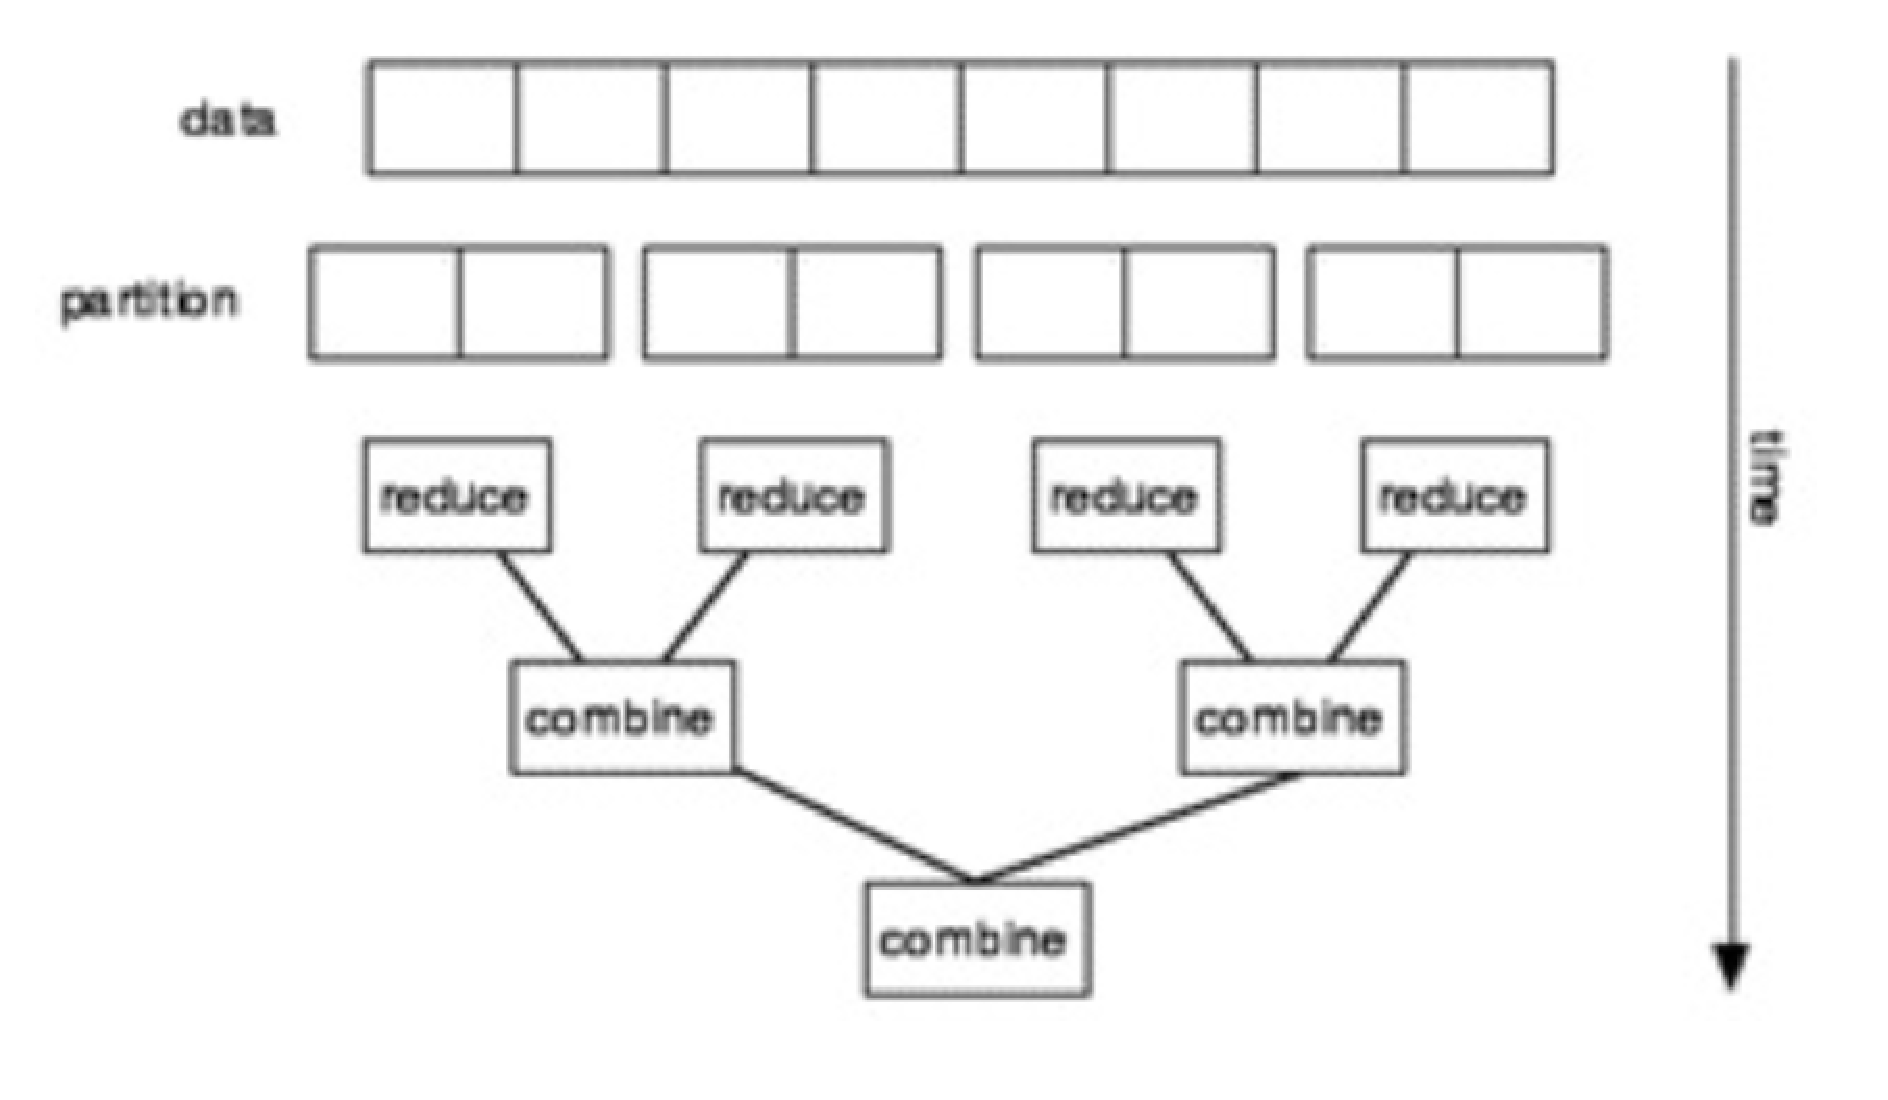
\includegraphics[width=12cm]{fig_05_005.eps}

先ほどの例に戻ると、\texttt{clojure.core.reducers}ライブラリを引き込み、reducerバージョンの関数を使って、ground-weightの計算を書き直すことができます。

\begin{lstlisting}[numbers=none]
(ns shipping.reducer
  (:require [shipping.domain :refer (ground?)]
            [clojure.core.reducers :as r]))

(defn ground-weight [products]
  (->> products
       (r/filter ground?)
       (r/map :weight)
       (r/fold +)))
\end{lstlisting}

この実装は、\texttt{clojure.core} 名前空間の代わりに \texttt{clojure.core.reducers} 名前空間の関数を使用する以外は、オリジナルバージョンと同様です。reducersの主な利点の1つは、他のアプローチと比較して、操作の構成可能な形状を維持することができることです。

フィルタとマップのリデューサーのバージョンは、元の積のベクトルに対して変換を実行しないことを思い出してください! 最終的に\texttt{fold}を呼び出すまで何も起こりません。この例では、reduceとcombineの両方のステージで同じ関数を使用する、最も単純なバージョンの\texttt{fold}を使用しています。

問題を再帰的に分割する並列計算では、以下のタイミングを決定する必要があります。分割と再合成は、単に作業を行うよりもコストがかかります。これは個々の計算の大きさに依存するため、最適な答えはない。\texttt{fold}関数では、分割サイズを指定することができ、デフォルトはグループあたり512要素(\texttt{+}などの単純な算術演算でうまくいくサイズ)です。より複雑な変換を行う場合は、より小さなパーティションサイズが有効でしょう。

今回はマルチコアマシンでのパフォーマンスを向上させるためにリデューサを使用するので、シーケンスとリデューサのパフォーマンスを比較してみましょう。

\subsection{Reducerの性能}

シーケンス版とリデューサ版を、どんどん大きな商品のベクターで走らせてみます。詳細を理解するために、2つのスケールでデータを見ることにします。次の図は、商品数(N)が32、128、512、2,048の場合の結果です。デフォルトのパーティションサイズは512なので、N <= 512の場合、実際には折りたたみは並列ではなく、1つのパーティションになります。これらのテストは、4つのハイパースレッドコア(8コアとして報告)を持つMacBook Proで実行されました。

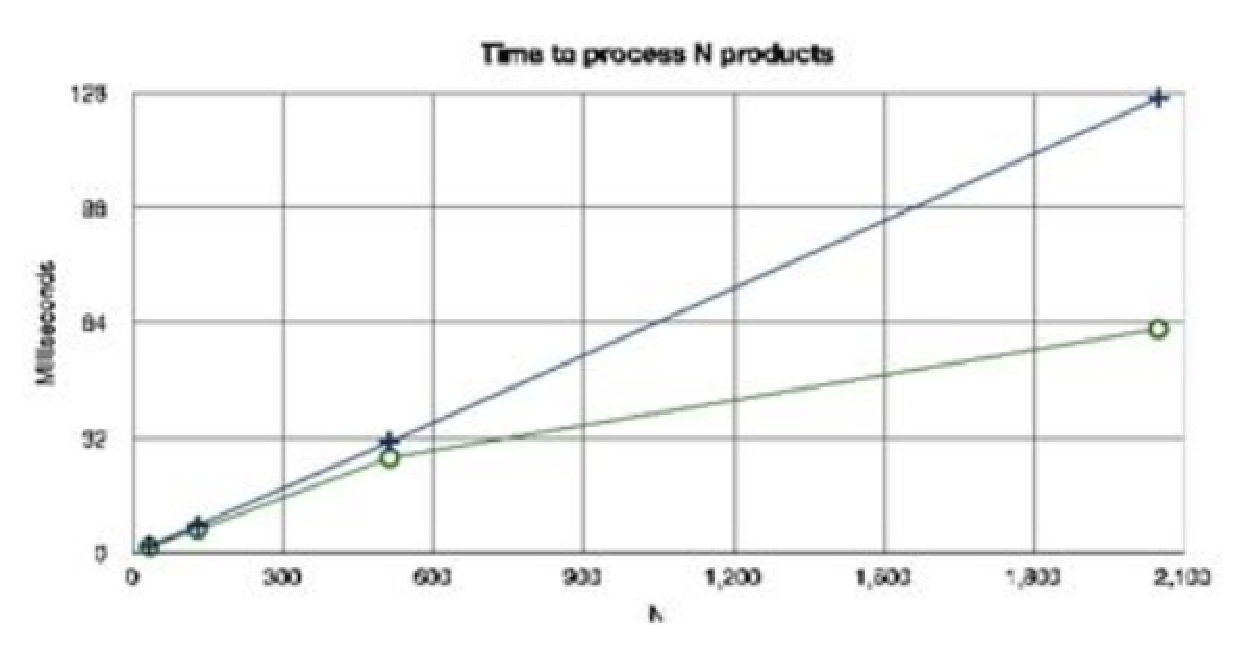
\includegraphics[width=10cm]{fig_05_006.eps}

予想通り、N=512まではシーケンス版とリデューサーの性能は同等である。しかし、パーティションサイズを超えると、シーケンス版はシングルスレッドですが、リデューサ版はデータをパーティションに分割し、異なるスレッドで並列実行されます。ここで一旦引いて、次の図にある3つのデータポイント(N=8,192, 32,768, 131,072)を追加して、Nの値が大きい場合の影響を見てみましょう。

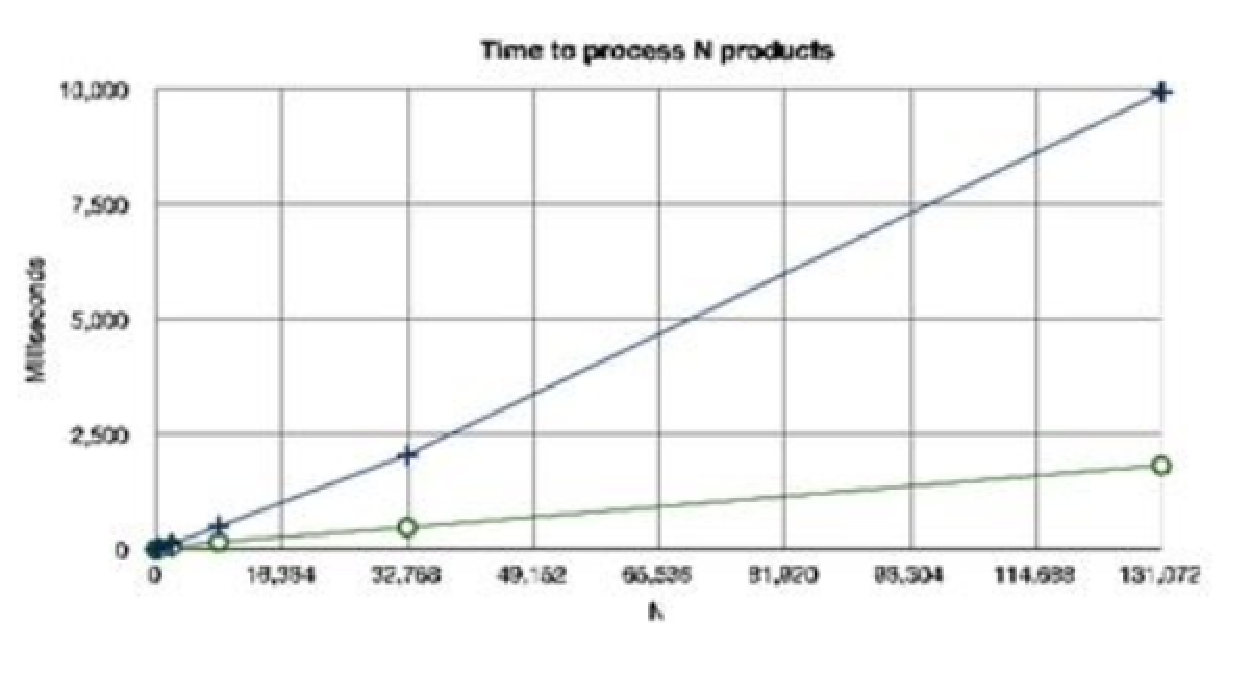
\includegraphics[width=10cm]{fig_05_007.eps}

Nが大きくなると、reducerの利点が明らかになる。reducerは4つの利用可能なコアに作業を分割するのに対し、シーケンスバージョンは1つのコアを使用するのである。さらに、reducer版ではゴミの発生が少ないので、ガベージコレクタの負荷が軽減されます。

reducerの主な利点の1つは、より多くのコアを持つマシンに移行したときに、同じコードがより速く実行されることです。マシンのコアの一部をオフにすることで、その違いをシミュレートすることができます。N=131,072 を固定し、コア数を変化させながら、シーケンスとreducerのテストを再実行してみましょう。このテストでは、ハイパースレッディングもオフにして、その影響を排除しています。

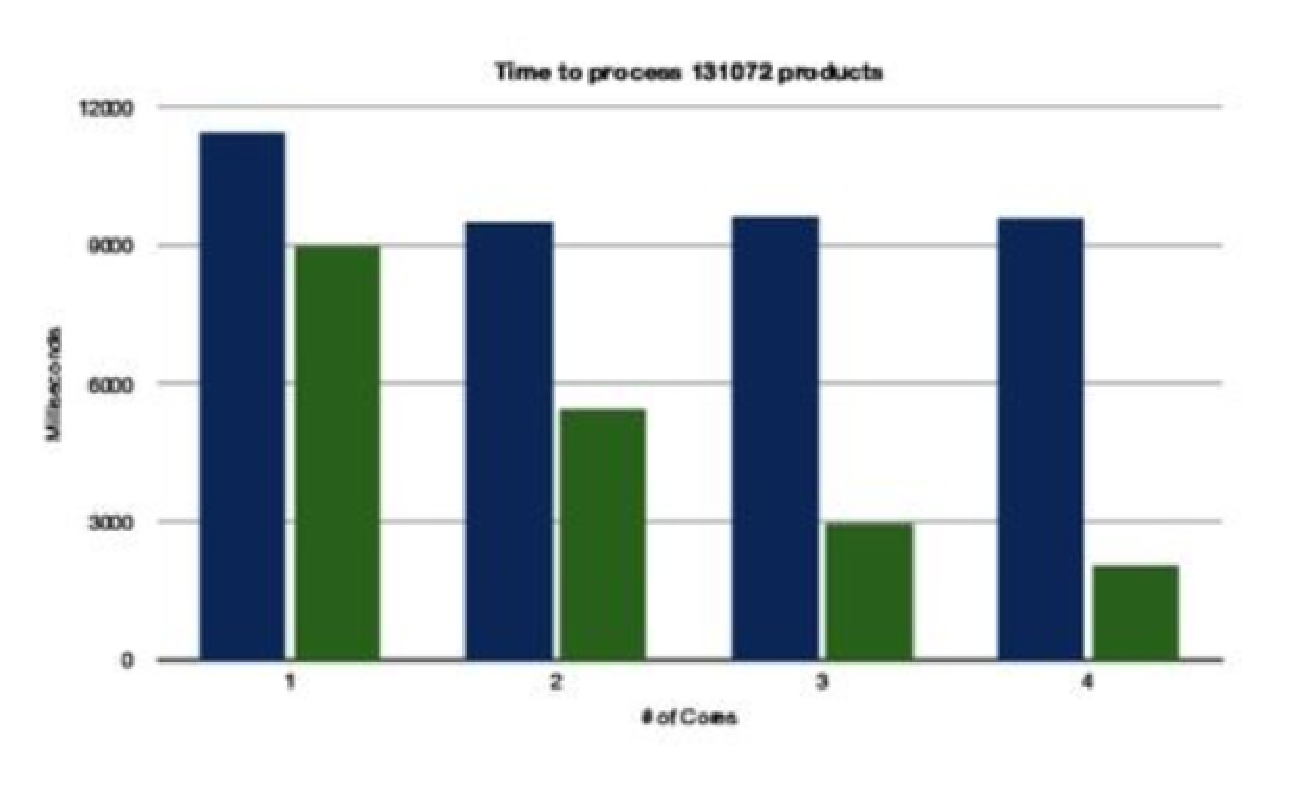
\includegraphics[width=10cm]{fig_05_008.eps}



前の図で、シーケンス版の性能はコア数に関係なく事実上同じであることがお分かりいただけると思います。シングルコアの場合は、ガベージコレクションやその他のマシン上の作業も唯一のコアを使用するため、特に悪化します。しかし、reducer版では、明らかに余分なコアの恩恵を受けており、同じコードが自動的に高速化されます。8コアや16コアのサーバーに移行すれば、このコードはさらに高速になると推測できます。

reducerを使うときは、データの大きさ、パーティションごとの作業の大きさ、想定するコア数を考えることが重要です。要素数がパーティションサイズより小さいときは、シングルスレッドになります(それでも穏やかな効果が見られるかもしれません)。パーティションサイズを超えると、reducerはマルチスレッドになりますが、オーバーヘッドが発生するため、コア数の倍数にはならない可能性があります。

もう1つのキーは、並列折りたたみ可能なコレクションは(現在ではもっと追加されるかもしれませんが)永続ベクトルと永続マップだけであることです。他のすべてのコレクション(およびシーケンス)は、1つのパーティション上のリダクションにフォールバックされます。このリダクションはより高速になる可能性がありますが、マルチスレッドにはなりません。

Reducerは、シーケンスライブラリの使いやすさと、fork/joinのマルチスレッド性能を併せ持つもので、両者の良いとこ取りのようなものです。reducers を最大限に活用するには、処理量が多く、データが折りたたみ可能なベクトルやマップとして存在する場合に限定して使用するようにしましょう。